\documentclass[12pt]{article}
\usepackage[utf8]{inputenc}
\usepackage{graphicx}
\usepackage{amsmath, amssymb}
\usepackage{hyperref}
\usepackage{geometry}
\usepackage{natbib}

\geometry{margin=1in}

\title{Data-Centric Federated Learning Framework for Predictive Maintenance of Wind Energy Turbines}
\author{Yassire Ammouri \\ Mohammed V University, Rabat}
\date{}

\begin{document}

\maketitle

\begin{abstract}
This paper presents...
\end{abstract}

\textbf{Keywords:} Federated Learning, Predictive Maintenance, Wind Turbines, Industrial IoT, Privacy

\section{Introduction}
\subsection{Problem Statement }
Predictive Maintenance tasks in an operational environment such as the one of Wind Turbine can be very challenging due to various constraints, mainly about the data. Operational data of WT systems present various issues, first the failures sample are very rare compared to the normal operational data samples, which makes the data very unbalanced, the balance rate may up sometimes to more than 80, and that's very crucial when dealing with Predictive maintenance model, cuz they required enough fault data samples in order to well learn degradation and failure patterns . Second, the dimensionality of the data is very large, talking about more than 100 features in most of the publicly available datasets which require proper feature selection and engineering. Also, the lack of good quality open access operational WT datasets makes the task of applying robust Predictive Maintenance systems more complex and harder. All this pushes researchers to leave Predictive Maintenance behind and go with Fault and Anomaly Detection with more focus on Model-Centric approaches.


% \section{Methodology: A Data-Centric Federated Learning Framework}

% This section details the proposed \textbf{Data-Centric Federated Learning (DCFL) framework} developed to overcome the challenges facing the application of predictive maintenance tasks in operational and critical system environments like that of wind energy such as data privacy, statistical heterogeneity (Non-IID data), and severe class imbalance inherent in real-world wind turbine (WT) predictive maintenance (PdM). The methodology pivots from a traditional model-centric approach to prioritize a rigorous, systematic data preparation pipeline, ensuring the learning algorithm is applied to high-quality, domain-specific supervisory signals.

% \subsection{Data Acquisition and Problem Formulation}

% \subsubsection{Dataset Selection and Prediction Task}
% The experiments utilize the publicly available \textbf{EDP Open Data (2016/2017) dataset}, selected specifically because it provides operational Supervisory Control and Data Acquisition (SCADA) signals, Meteorological Mast (MetMast) data, and corresponding historical failure logbooks across four unique turbines (T01, T06, T07, T11).\\

% The objective is formulated as a \textbf{multi-class time-series classification task} designed for fault diagnosis. The model is required to classify the operational state of the turbine into one of six distinct categories: Normal Operation (Class 0) and five component-specific failure modes (Gearbox, Transformer, Generator, Generator Bearing, and Hydraulic Group).

% \subsubsection{Distributed Architecture and Data Partitioning}
% The system employs a \textbf{Horizontal Federated Learning (HFL)} architecture, simulating a collaborative wind farm deployment where raw data remains local to each turbine.
% \begin{itemize}
%     \item \textbf{Clients (Training Participants):} Three individual wind turbines (T01, T06, T07) are designated as federated clients, each maintaining its unique, private partition of processed data.
%     \item \textbf{Centralized Evaluation Set:} Data from the fourth turbine (\textbf{T11}) is entirely reserved by the central server for unbiased evaluation of the global model after each aggregation round. This ensures that performance metrics reflect the model's generalization capability on completely unseen, heterogeneous industrial data.
% \end{itemize}

% This natural partitioning scheme results in a demonstrably \textbf{Non-Independent and Identically Distributed (Non-IID) scenario} where clients exhibit differing data quantities, operational characteristics, and distinct class distributions of failure events, mirroring real industrial operations.

% \subsubsection{The Data-Centric Pipeline (DC-Pipeline)}

% The DCFL methodology focuses on solving the data quality issues (label inaccuracy, excessive dimensionality, and imbalance) prior to model training. The pipeline transforms raw data through three systematic steps.

% \paragraph{Temporal Label Generation via Dynamic Failure Windowing}
% To accurately generate pre-failure supervisory signals, a \textbf{Dynamic Failure Window Labeling Strategy} was implemented using the Historical Failure Logbook as ground truth. This strategy aligns SCADA samples with component-specific degradation timelines, adhering to Prognostics and Health Management (PHM) best practices.
% \begin{itemize}
%     \item \textbf{Objective:} Label data points as pre-failure conditions within a specific time window preceding the recorded failure event.
%     \item \textbf{Component-Specific Windows:} The duration is based on domain knowledge of component degradation rates:
%     \begin{itemize}
%         \item \textbf{Gearbox and Generator Bearing:} 72 hours (based on incremental temperature rise).
%         \item \textbf{Hydraulic Systems:} 48 hours (based on gradual pressure changes).
%         \item \textbf{Electrical Systems (Transformer and Generator):} 24 hours (due to more instantaneous fault characteristics).
%     \end{itemize}
% \end{itemize}

% \paragraph{Feature Engineering and Dimensionality Reduction}
% The initial dataset comprises over 120 features (83 SCADA variables and 40 MetMast variables). To improve computational efficiency across distributed clients and mitigate overfitting, the feature space was systematically reduced through domain knowledge and correlation analysis.
% \begin{itemize}
%     \item \textbf{Final Feature Set:} The resulting dataset utilizes \textbf{26 highly relevant features}, focusing on critical parameters (Temperature, Rotational Speed, Power Production, and Dynamic Load Signals) confirmed by literature to be key indicators for mechanical and electrical degradation.
%     \item \textbf{Preprocessing:} All features were subjected to standard data cleaning (outlier removal, handling of missing values) and normalization to ensure stable training convergence for the neural network architecture.
% \end{itemize}

% \paragraph{Correcting Severe Class Imbalance}
% The processed dataset exhibits extreme class imbalance (approximately 98\% Normal operation, $\approx$2\% distributed across five rare fault types). This challenge was addressed by a dual strategy:

% \begin{enumerate}
%     \item \textbf{TimeGAN-based Minority Augmentation:} \textbf{Time-series Generative Adversarial Networks (TimeGAN)} were employed to synthesize high-fidelity time-series samples for the rare fault classes. This technique ensures that the generated data maintains the crucial temporal dependencies inherent in degradation sequences, validated using PCA and t-SNE.
%     \item \textbf{Intelligent Downsampling:} A custom, time-concerned downsampling strategy was applied to the majority (Normal) class to preserve sequential context while achieving a balanced distribution, resulting in a final training dataset of approximately 50,000 rows.
% \end{enumerate}
% ```latex
% \subsection{Federated Learning Workflow}
% \label{subsec:fl_workflow}

% The DCFL framework executes an iterative collaborative training protocol spanning multiple federated rounds. Each round $t \in \{1, 2, \ldots, T\}$ comprises seven sequential phases that collectively enable privacy-preserving distributed learning while handling the statistical heterogeneity inherent in wind turbine operational data. The protocol ensures that no raw SCADA measurements leave client premises, with only compressed model parameter updates traversing the network.

% \begin{enumerate}
%     \item \textbf{Initialization and Client Selection:} 
%     At the commencement of training ($t=0$), the central coordination server instantiates the global 1DCNN-BiLSTM model with parameters $\omega_{global}^{0}$ initialized using Xavier uniform distribution to ensure stable gradient flow during early training phases. These initial weights are broadcast to all registered client nodes via secure communication channels.
    
%     For subsequent rounds ($t \geq 1$), the server implements an adaptive client selection mechanism to optimize convergence under resource constraints. The selection strategy evaluates each client $k$ based on two criteria: (i) \textit{data contribution quality}, quantified by the validation loss reduction $\Delta \mathcal{L}_k$ achieved in previous rounds, and (ii) \textit{computational reliability}, measured by the client's historical participation consistency and training completion rate. Formally, client selection probability is defined as:
%     \begin{equation}
%     p_k^{(t)} = \frac{\exp(-\beta \cdot \Delta \mathcal{L}_k^{(t-1)}) \cdot \mathbb{I}[\text{reliability}_k > \tau]}{\sum_{j=1}^{K} \exp(-\beta \cdot \Delta \mathcal{L}_j^{(t-1)}) \cdot \mathbb{I}[\text{reliability}_j > \tau]}
%     \label{eq:client_selection}
%     \end{equation}
%     where $\beta$ controls selection aggressiveness, $\tau$ is the minimum reliability threshold, and $\mathbb{I}[\cdot]$ is the indicator function. This probabilistic selection ensures that turbines demonstrating consistent training contributions and informative data distributions receive priority in bandwidth-constrained scenarios, while maintaining diversity to prevent convergence to local optima dominated by a subset of clients.
    
%     \item \textbf{Local Data Preparation:} 
%     Upon receiving the global model parameters $\omega_{global}^{t}$, each selected client $k \in \mathcal{S}^{(t)}$ (where $\mathcal{S}^{(t)}$ denotes the set of participating clients in round $t$) independently executes the complete data-centric preparation pipeline on its private SCADA partition $\mathcal{D}_k$. This preprocessing operates entirely within the client's secure computational perimeter and encompasses four critical transformations:
    
%     \begin{itemize}
%         \item \textit{Dynamic temporal labeling}: Application of component-specific failure windows ($w_c \in \{72h, 48h, 24h\}$ for bearings, hydraulics, and electrical systems respectively) to propagate failure event labels backward in time, creating supervisory signals that capture pre-failure degradation patterns.
        
%         \item \textit{Physics-informed feature selection}: Dimensionality reduction from 123 raw SCADA and meteorological variables to 26 domain-relevant features through correlation thresholding ($|\rho_{ij}| > 0.95$ triggers redundancy elimination) and retention of thermodynamic indicators, rotational dynamics, and electrical production parameters known to correlate with mechanical degradation.
        
%         \item \textit{Class imbalance mitigation}: Sequential application of TimeGAN-based synthetic minority oversampling (generating temporally coherent failure sequences until minority classes reach $\approx$50\% of majority class count) followed by intelligent downsampling that preserves 30-day pre-failure windows while reducing normal operation samples by 85\%, yielding a balanced dataset with near-uniform class distribution.
        
%         \item \textit{Temporal windowing and normalization}: Construction of fixed-length sequences comprising 144 consecutive 10-minute intervals (24-hour operational windows) with feature-wise standardization ($\mu=0, \sigma=1$) computed exclusively from training partition statistics to prevent information leakage.
%     \end{itemize}
    
%     The prepared dataset $\tilde{\mathcal{D}}_k$ remains strictly local throughout this process, with preprocessing statistics (means, variances, synthetic sample metadata) never transmitted to the coordination server or peer clients.
    
%     \item \textbf{Local Model Training:} 
%     Each client initializes its local model $\mathcal{M}_k$ with the distributed global parameters: $\omega_k^{(t,0)} \leftarrow \omega_{global}^{t}$. Local training proceeds for $E$ epochs specified by the server, optimizing the model on the prepared dataset $\tilde{\mathcal{D}}_k$ through mini-batch stochastic gradient descent.
    
%     The local objective function incorporates class-weighted categorical cross-entropy to address severe class imbalance:
%     \begin{equation}
%     \mathcal{L}_k(\omega) = -\frac{1}{N_k}\sum_{i=1}^{N_k} \sum_{c=1}^{6} w_c \cdot y_{ic} \log\left(\hat{y}_{ic}(\omega)\right) + \frac{\lambda}{2}\|\omega\|_2^2
%     \label{eq:local_loss}
%     \end{equation}
%     where $N_k = |\tilde{\mathcal{D}}_k|$ is the client's dataset size, $w_c = N_k/(6 \cdot n_{kc})$ represents inverse-frequency class weights ensuring rare failure classes receive higher misclassification penalties, and $\lambda$ is the L2 regularization coefficient preventing overfitting to client-specific patterns.
    
%     Training employs the Adam optimizer with learning rate $\alpha = 0.001$, batch size $B = 64$, and early stopping with patience $p = 5$ epochs. To handle non-IID data distributions and prevent local models from diverging excessively from the global model, training incorporates proximal regularization:
%     \begin{equation}
%     \mathcal{L}_k^{\text{prox}}(\omega) = \mathcal{L}_k(\omega) + \frac{\mu}{2}\|\omega - \omega_{global}^{t}\|_2^2
%     \label{eq:proximal_loss}
%     \end{equation}
%     where $\mu = 0.1$ balances local adaptation against global consistency. This proximal term constrains parameter drift, ensuring clients with extreme data distributions (e.g., turbines with predominantly single-component failures) remain aligned with the collaborative global model capturing fleet-wide failure patterns.
    
%     Upon completing $E$ local epochs, the client computes the parameter update:
%     \begin{equation}
%     \Delta\omega_k^{(t)} = \omega_k^{(t,E)} - \omega_{global}^{t}
%     \label{eq:parameter_delta}
%     \end{equation}
%     representing the accumulated learning from local training, which is then privatized before transmission to the server.

%     \item \textbf{Privacy-Preserving Gradient Perturbation:} 
%     Before transmitting model updates to the coordination server, each client applies differential privacy mechanisms to provide formal privacy guarantees. The perturbation protocol comprises two sequential operations:
    
%     \textit{Gradient Clipping:} The parameter update is clipped to a maximum L2 norm to bound sensitivity:
%     \begin{equation}
%     \tilde{\Delta\omega}_k^{(t)} = \Delta\omega_k^{(t)} \cdot \min\left(1, \frac{C}{\|\Delta\omega_k^{(t)}\|_2}\right)
%     \label{eq:gradient_clipping}
%     \end{equation}
%     where $C = 1.0$ is the clipping threshold, ensuring that any single sample's contribution is bounded.
    
%     \textit{Calibrated Noise Injection:} The clipped update is perturbed with Gaussian noise:
%     \begin{equation}
%     \hat{\Delta\omega}_k^{(t)} = \tilde{\Delta\omega}_k^{(t)} + \mathcal{N}\left(0, \sigma^2 I\right), \quad \sigma = C \cdot z
%     \label{eq:noise_injection}
%     \end{equation}
%     where $z = 0.8$ is the noise multiplier. This provides $(\epsilon, \delta)$-differential privacy with $\epsilon = 5.0$ and $\delta = 10^{-5}$, computed via moments accountant across all training rounds. The privatized update $\hat{\Delta\omega}_k^{(t)}$ is transmitted via encrypted channels with typical message sizes of 2-5 MB, representing a 1000$\times$ reduction compared to raw SCADA data transmission.
    
%     \item \textbf{Federated Aggregation and Global Model Update:} 
%     The coordination server aggregates received updates $\{\hat{\Delta\omega}_k^{(t)}\}_{k \in \mathcal{S}^{(t)}}$ using weighted averaging:
%     \begin{equation}
%     \omega_{global}^{t+1} = \omega_{global}^{t} + \eta \cdot \sum_{k \in \mathcal{S}^{(t)}} \frac{n_k}{\sum_{j \in \mathcal{S}^{(t)}} n_j} \hat{\Delta\omega}_k^{(t)}
%     \label{eq:federated_aggregation}
%     \end{equation}
%     where $\eta = 1.0$ is the global learning rate, and $n_k / \sum_j n_j$ are normalized dataset size weights ensuring turbines with richer operational histories exert proportionally greater influence. The proximal regularization from Eq.~\ref{eq:proximal_loss} implicitly constrains this aggregation, preventing divergence from extreme data distributions. Critically, the server performs only linear weighted averaging on parameters—never accessing raw data, intermediate activations, or sample-level gradients.
    
%     \item \textbf{Centralized Global Model Evaluation:} 
%     The server evaluates the updated global model $\omega_{global}^{t+1}$ on held-out validation partition $\mathcal{D}_{\text{val}}$ (Turbine T11) for three purposes: (i) convergence detection via early stopping when accuracy plateaus for 10 consecutive rounds, (ii) generalization assessment on unseen turbine configurations through overall accuracy, macro-averaged F1-score, and per-class precision/recall, and (iii) model checkpointing:
%     \begin{equation}
%     \text{if } \text{acc}_{\text{val}}(\omega_{global}^{t+1}) > \max_{i < t+1} \text{acc}_{\text{val}}(\omega_{global}^{i}) \implies \text{save}(\omega_{global}^{t+1})
%     \label{eq:checkpointing}
%     \end{equation}
%     ensuring the best-performing model is retained for deployment.
    
%     \item \textbf{Model Redistribution and Round Completion:} 
%     The refined global parameters $\omega_{global}^{t+1}$ are broadcast to all registered clients:
%     \begin{equation}
%     \omega_k^{(t+1,0)} \leftarrow \omega_{global}^{t+1}, \quad \forall k \in \{1, \ldots, K\}
%     \label{eq:model_redistribution}
%     \end{equation}
%     This ensures even non-participating clients benefit from collaborative knowledge and can utilize the updated model for local inference. The server logs round completion metadata (participating clients, training loss, validation metrics, communication statistics) for post-hoc analysis.
% \end{enumerate}


% \subsection{Predictive Model Architecture}

% \subsubsection{Hybrid 1DCNN-BiLSTM Design}
% The local predictive model implemented on each client is a custom-designed \textbf{1D Convolutional Neural Network--Bidirectional Long Short-Term Memory (1DCNN-BiLSTM)} hybrid network, selected for its proficiency in processing multivariate temporal data.

% \begin{itemize}
%     \item \textbf{Input Configuration:} The model accepts an input tensor of \textbf{144 timesteps} across \textbf{28 features} (the 26 selected SCADA/MetMast variables plus time context). This window represents a 24-hour lookback period (at 10-minute intervals), providing sufficient context for fault prediction.
%     \item \textbf{Feature Extraction (1DCNN):} Sequential 1D Convolutional layers are utilized to automatically extract spatial features and localized patterns across the multiple sensor inputs within each timestep, capturing invariant characteristics of the signals.
%     \item \textbf{Temporal Modeling (BiLSTM):} The extracted features are fed into a stack of \textbf{Bidirectional Long Short-Term Memory (BiLSTM)} layers. BiLSTM layers process the sequence both forwards and backwards, effectively capturing long-distance temporal dependencies and modeling the evolving degradation patterns leading up to a failure event.
%     \item \textbf{Training Objective:} The model utilizes a \textbf{class-weighted loss function} to ensure that all six classes contribute proportionally to the learning process, minimizing the impact of any residual imbalance.
% \end{itemize}

% \subsection{Federated Learning System Implementation}

% \subsubsection{Distributed Architecture and Technology Stack}
% The entire system is deployed within a containerized environment using \textbf{Docker Compose} to ensure robust and reproducible environment isolation. The collaborative learning is orchestrated by the \textbf{Flower (flwr v1.18.0) framework}.

% \begin{itemize}
%     \item \textbf{Server Side:} The \textit{ServerApp} (coordinator) and \textit{SuperLink} (communication manager) manage the federated training rounds, model parameter aggregation, and global evaluation.
%     \item \textbf{Client Side:} Each wind turbine (T01, T06, T07) is represented by a containerized \textit{ClientApp} (local training logic) running on a \textit{SuperNode}.
% \end{itemize}

% \subsubsection{Addressing Non-IID Data: FedProx Optimization}
% To maintain stable convergence despite the statistical heterogeneity across the client datasets, the central server employs a customized strategy extending the \textbf{Federated Proximal (FedProx)} algorithm.
% \begin{itemize}
%     \item \textbf{Mechanism:} FedProx introduces a proximal term ($\mu$) to the local objective function. This term penalizes local model updates that deviate excessively from the global model parameters, thereby mitigating ``client drift'' which commonly leads to instability and performance degradation in Non-IID settings.
%     \item \textbf{Training Configuration:} The synchronous training setup runs for \textbf{50 global rounds}, with \textbf{5 local epochs} performed by 100\% of participating clients per round (fraction-fit = 1.0).
% \end{itemize}

% \subsubsection{Privacy Enhancement: Differential Privacy (DP) Integration}
% To provide formal, mathematical assurance of data confidentiality beyond the inherent data locality of FL, \textbf{Differential Privacy (DP)} is integrated client-side.
% \begin{itemize}
%     \item \textbf{DP Mechanism:} Before transmitting model updates to the central server, two steps are applied to the local gradients:
%     \begin{enumerate}
%         \item \textbf{Gradient Clipping:} The L2 norm of the gradients is clipped to a defined threshold (e.g., $l2\_norm\_clip$), limiting the maximum influence of any single data batch.
%         \item \textbf{Noise Addition:} Calibrated Gaussian noise is added to the clipped gradients, controlled by a specific noise multiplier. This perturbation makes it computationally infeasible for an adversary to reconstruct private training data points from the shared model updates.
%     \end{enumerate}
% \end{itemize}

% \subsection{Experimental Protocol and Validation}

% \subsubsection{Performance Benchmark and Centralized Evaluation Protocol}
% To rigorously validate the efficacy of the proposed DCFL framework, a comparative protocol was established:

% \begin{enumerate}
%     \item \textbf{Centralized Benchmark:} The optimal performance achievable was established by training the identical 1DCNN-BiLSTM model on a fully aggregated, balanced dataset (the output of the DC-Pipeline). This acts as the upper bound for performance. The significant performance gain (from 84.3\% baseline accuracy to \textbf{99.8\%} data-centric accuracy in the centralized setting) quantitatively justifies the data-centric focus.
%     \item \textbf{Federated Evaluation:} The global model's performance during FL was assessed using the independent \textbf{T11 dataset}. This unseen data provides an unbiased measure of generalization, crucial for real-world reliability.
%     \item \textbf{Metrics:} Performance quantification focuses on robustness for the minority classes, utilizing \textbf{Precision, Recall, and F1-Score} (Macro-Average and class-specific) in addition to overall accuracy. Convergence stability is tracked using loss and accuracy curves.
% \end{enumerate}

% \subsubsection{Suggestion for Enhanced Methodological Transparency}

% For Q1/Q2 journal submissions, incorporating subsections that explicitly address system integrity and experimental tracking enhances confidence in the results:

% \begin{itemize}
%     \item \textbf{Monitoring and Reproducibility:} All training metrics, hyperparameters, and model checkpoints were recorded in real-time using \textbf{Weights \& Biases (W\&B)}. This rigorous experiment tracking ensures full reproducibility of both local and federated training dynamics.
%     \item \textbf{System and Resource Constraints:} High-impact papers often detail computational environments to contextualize performance trade-offs. It is essential to note that experiments were conducted on a resource-constrained environment (e.g., CPU execution due to GPU initialization errors), leading to moderate training times and high peak CPU/memory usage. This context validates the practical challenges faced when deploying complex models like 1DCNN-BiLSTM in distributed, edge-like settings.
% \end{itemize}

\subsection{Data-Centric Preparation Pipeline}
\label{subsec:dc_pipeline}

The data-centric preparation pipeline constitutes a fundamental component of the proposed framework, systematically transforming raw, unlabeled SCADA data into training-ready datasets suitable for federated predictive maintenance. This client-side preprocessing workflow addresses three endemic challenges in industrial failure prediction: sparse failure annotations, severe class imbalance, and high-dimensional sensor redundancy. Unlike conventional approaches that treat data preparation as a perfunctory preprocessing step, our methodology positions systematic data curation as the primary driver of model performance—demonstrating that properly curated datasets enable standard architectures to achieve superior predictive accuracy compared to sophisticated models trained on raw, unprocessed operational data.

\begin{figure}[htbp]
    \centering
    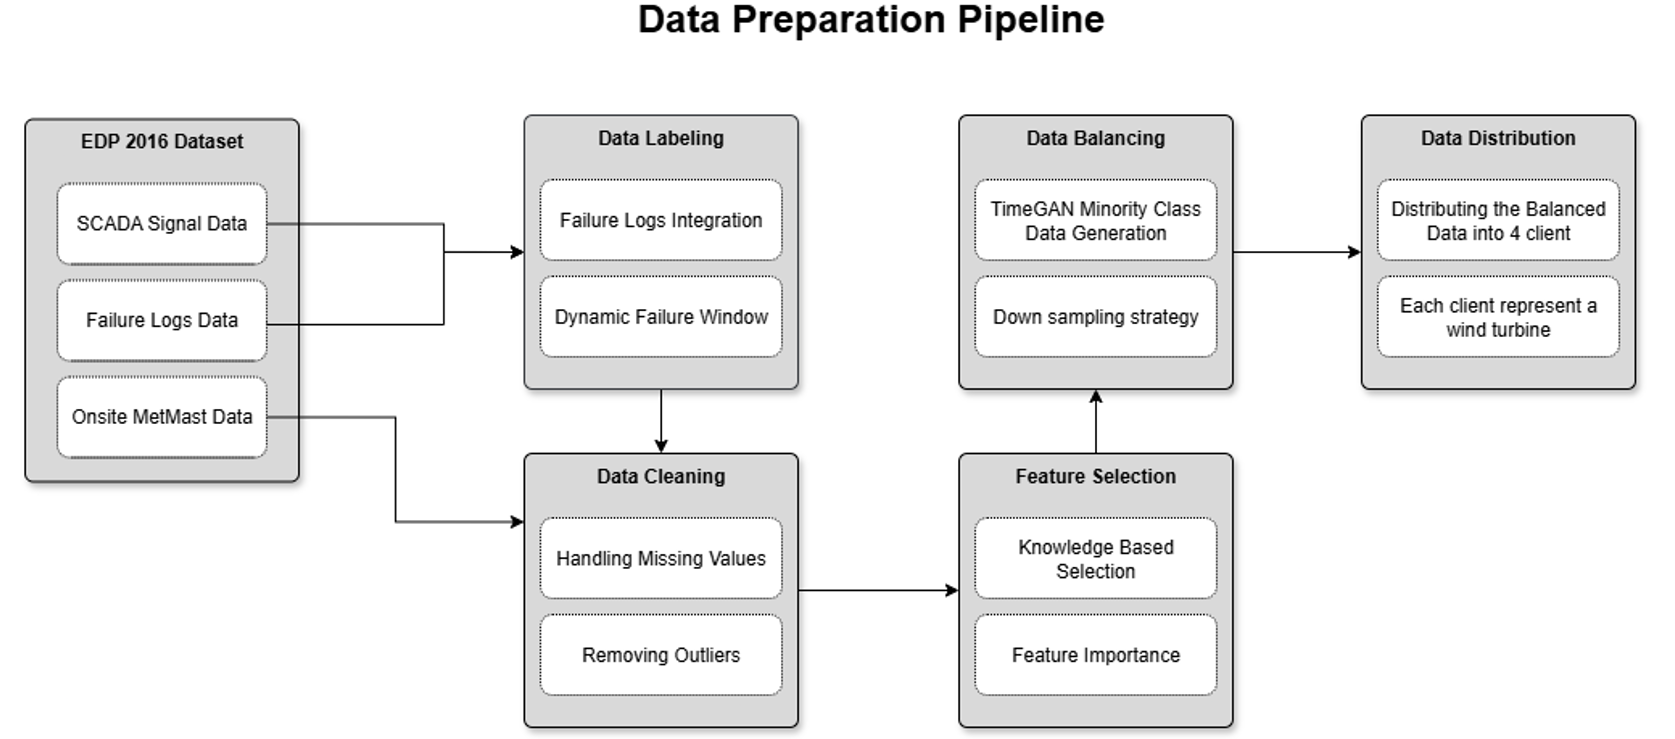
\includegraphics[width=0.75\linewidth]{img/DC_Pipeline.png}
    \caption{Data-centric preparation pipeline workflow showing sequential transformation from raw SCADA data to balanced, training-ready datasets through temporal labeling, feature selection, class balancing, and federated distribution stages.}
    \label{fig:dc_pipeline}
\end{figure}

The pipeline executes five sequential transformations, each addressing specific data quality limitations inherent in operational wind turbine monitoring systems.

\subsubsection{Dynamic Temporal Labeling Strategy}
\label{subsubsec:temporal_labeling}

The EDP dataset provides unlabeled SCADA time-series accompanied by a sparse failure logbook documenting 21 component-specific failure events across four turbines. Direct alignment of these point-in-time failure timestamps with SCADA measurements yields insufficient training samples for supervised learning—the 21 documented failures represent only 0.005\% of the 400,000+ operational records. To address this label scarcity while capturing pre-failure degradation patterns essential for predictive maintenance, we employ dynamic temporal windowing that propagates failure labels backward in time.

The labeling protocol operates by defining component-agnostic temporal windows preceding each documented failure event. All SCADA samples falling within these windows are assigned the corresponding fault class, transforming sparse failure events into extended pre-failure sequences that encode gradual degradation trajectories. To systematically evaluate the trade-off between prediction horizon and pattern capture adequacy, we implement two distinct labeling strategies:

\paragraph{Strategy 1: 30-Day Pre-Failure Window}
This conservative approach applies a 30-day (720-hour) pre-failure window coupled with a 1-day (24-hour) post-failure recovery window to each documented failure event. The rationale is twofold: (i) limiting the pre-failure window to one month reduces the risk of mislabeling normal operational variations as incipient faults, maintaining higher label precision, and (ii) the shorter horizon aligns with industry practices where maintenance interventions typically occur within 2-4 weeks of fault detection. However, this conservative windowing may inadequately capture early-stage degradation signatures for slowly developing mechanical failures (e.g., bearing wear, gearbox tooth pitting), potentially limiting the model's ability to provide extended advance warning.

Applying this strategy yields the class distribution presented in Table~\ref{tab:class_dist_30d}, with failure classes constituting approximately 19\% of labeled samples after windowing.

\begin{table}[htbp]
\centering
\caption{Class distribution under 30-day pre-failure windowing strategy}
\label{tab:class_dist_30d}
\begin{tabular}{lrr}
\toprule
\textbf{Class} & \textbf{Sample Count} & \textbf{Percentage} \\
\midrule
0 (Normal) & 335,902 & 80.5\% \\
1 (Gearbox) & 30,189 & 7.2\% \\
2 (Transformer) & 25,006 & 6.0\% \\
3 (Generator) & 12,886 & 3.1\% \\
4 (Generator Bearing) & 8,641 & 2.1\% \\
5 (Hydraulic Group) & 4,517 & 1.1\% \\
\midrule
\textbf{Total} & \textbf{417,141} & \textbf{100\%} \\
\bottomrule
\end{tabular}
\end{table}

\paragraph{Strategy 2: 60-Day Pre-Failure Window}
The extended approach doubles the pre-failure horizon to 60 days (1,440 hours) while maintaining the 1-day post-failure window. This aggressive labeling strategy prioritizes recall—capturing subtle, long-term degradation patterns that manifest weeks before catastrophic failure—at the cost of potentially increased false positive rates if early-window samples represent normal operational variations rather than true pre-failure states. The 60-day horizon is particularly justified for mechanical components exhibiting gradual degradation trajectories, such as gearbox bearing fatigue or generator winding insulation breakdown, where detectable anomalies may emerge 4-8 weeks before functional failure.


The resulting class distribution (Figure~\ref{fig:class_dist_60d}) demonstrates substantially increased failure class representation, with fault samples constituting approximately 42\% of the labeled dataset.

\begin{figure}[htbp]
    \centering
    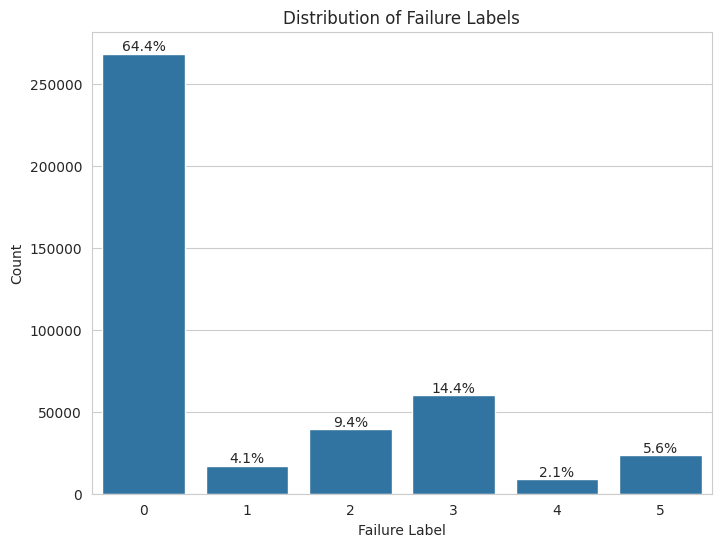
\includegraphics[width=0.7\linewidth]{img/class_distribution_60d.png}
    \caption{Class distribution under 60-day pre-failure windowing strategy, showing increased failure class representation compared to 30-day strategy.}
    \label{fig:class_dist_60d}
\end{figure}

\begin{table}[htbp]
\centering
\caption{Class distribution under 60-day pre-failure windowing strategy}
\label{tab:class_dist_60d}
\begin{tabular}{lrr}
\toprule
\textbf{Class} & \textbf{Sample Count} & \textbf{Percentage} \\
\midrule
0 (Normal) & 268,559 & 58.1\% \\
1 (Gearbox) & 17,094 & 3.7\% \\
2 (Transformer) & 39,295 & 8.5\% \\
3 (Generator) & 60,036 & 13.0\% \\
4 (Generator Bearing) & 8,810 & 1.9\% \\
5 (Hydraulic Group) & 23,347 & 5.0\% \\
\midrule
\textbf{Total} & \textbf{417,141} & \textbf{100\%} \\
\bottomrule
\end{tabular}
\end{table}

\paragraph{Strategy 3 : Dinamic Failure Window}
the thirst strategy tested for the labeling process is using a component specific pre-failure window. each WT component has different failure indication and periodes, so using a static failure window for all the failure types may not be sefficient. so based on the letterature and domain knowledge we gathered informations related every component pre-failure signiture and we use it to label the data. 

\paragraph{Post-Failure Window Detection}

While pre-failure windows are commonly used to capture degradation patterns leading to component failures, post-failure periods are often neglected in the labeling process. However, as illustrated in Figure~\ref{fig:post_failure}, wind turbines do not immediately return to normal operational conditions after a failure occurs. A recovery period exists during which the system exhibits abnormal behavior due to maintenance activities, component replacement, and system recalibration. Failing to account for these post-failure windows introduces label noise, as data points during recovery are incorrectly labeled as ``healthy,'' potentially degrading model performance. Therefore, we developed a data-driven methodology to determine appropriate post-failure windows for each component type.

\textbf{Baseline Establishment and Recovery Detection.} For each failure event in the logbook, we first establish a pre-failure operational baseline by analyzing data from 30 days before failure occurrence, excluding the last 24 hours to avoid early degradation patterns. We focus exclusively on operational periods (Power $> 0$) and calculate statistical measures for key signals: generator RPM, power output, and wind speed. For each signal, we compute the mean ($\mu$), standard deviation ($\sigma$), and interquartile ranges ($Q_{25}$, $Q_{75}$).

We then employ a dual-method approach to detect recovery: (1) \textit{Signal Stabilization} -- monitoring when operational signals return to baseline range $[\mu - \sigma, \mu + \sigma]$ and remain stable for at least 6 consecutive hours (36 measurements), ensuring temporary fluctuations are not mistaken for full recovery; (2) \textit{Zero-Output Analysis} -- identifying extended periods of zero power output immediately after failure and detecting when consistent power generation resumes, indicating the turbine has been repaired and returned to service.

\textbf{Component-Specific Window Calculation.} After detecting recovery times for all failures in the dataset, we aggregate results by component type (Generator, Gearbox, Transformer, Generator Bearing, Hydraulic Group). For each component, we calculate recovery duration statistics: mean, median, standard deviation, and percentiles. The recommended post-failure window for each component is determined as:

\begin{equation}
W_{\text{post}} = \max(P_{75}, \mu + \sigma)
\end{equation}

where $P_{75}$ is the 75th percentile of recovery durations, $\mu$ is the mean, and $\sigma$ is the standard deviation. This conservative approach ensures that 75\% of observed recovery periods are captured while accounting for variability through the mean-plus-standard-deviation criterion. The final window is rounded up to the nearest 12 hours for practical implementation. Table~\ref{tab:post_failure_windows} summarizes the derived post-failure windows for each component type, which are subsequently used in the target variable generation process.


\paragraph{Comparative Evaluation Protocol}
To empirically determine the optimal labeling strategy, we train identical 1DCNN-BiLSTM architectures on datasets derived from the combinations of the previously listed windowing approaches, evaluating performance on a held-out test partition (Turbine T11) that undergoes identical labeling transformations. The comparative analysis examines: (i) overall classification accuracy across all six operational states, (ii) macro-averaged F1-score to account for residual class imbalance, (iii) per-class recall for each fault type (critical for assessing the model's ability to detect rare but catastrophic failures), and (iv) prediction horizon—the average lead time between model fault detection and actual failure occurrence, computed from true positive predictions.

The selected labeling strategy (determined through experimental validation in Section~\ref{sec:results}) is then consistently applied across all federated clients to ensure uniform supervisory signal generation throughout the distributed training process.

% \subsubsection{Feature Engineering and Selection}
% \label{subsubsec:feature_selection}
% Raw wind turbine monitoring systems capture extensive operational and environmental parameters, with the merged SCADA-MetMast dataset comprising 123 variables (83 turbine sensors + 40 meteorological measurements). This high-dimensional feature space introduces three challenges for federated learning: (i) computational overhead during local training, (ii) increased risk of overfitting to client-specific noise rather than generalizable failure patterns, and (iii) communication bandwidth consumption when transmitting gradient updates for unnecessarily large parameter spaces.

% To address these limitations while preserving predictive information, we implement a hybrid feature selection methodology combining domain expertise with statistical redundancy analysis:

% \paragraph{Correlation-Based Redundancy Elimination}
% We compute the Pearson correlation matrix across all 123 variables, identifying feature pairs exhibiting correlation coefficients $|\rho_{ij}| > 0.95$. Within each highly correlated cluster, we retain the variable with strongest physical interpretability based on wind turbine engineering principles, eliminating derived or redundant measurements. For example, among multiple temperature sensors monitoring the same bearing assembly, we retain the sensor positioned closest to the critical load zone while excluding auxiliary measurements.

% \paragraph{Physics-Informed Feature Retention}
% Guided by established wind turbine prognostics literature and domain expertise, we prioritize variables with documented relationships to specific failure mechanisms. The selection emphasizes thermodynamic indicators (bearing temperatures, oil temperatures) that correlate with mechanical wear, rotational dynamics (RPM measurements) revealing drivetrain imbalances, electrical production parameters (power output, voltage phases) detecting generator degradation, and control signals (pitch angles, yaw positions) characterizing dynamic loading conditions. Environmental variables from the MetMast dataset—including wind speed, direction, ambient temperature, humidity, and atmospheric pressure—provide critical contextual normalization, distinguishing operational anomalies from weather-induced variations.

% This hybrid approach reduces dimensionality from 123 to 26 features while maintaining comprehensive coverage of the physical systems implicated in wind turbine failures. Table~\ref{tab:feature_categorization} organizes the retained features by turbine subsystem, demonstrating balanced representation across mechanical, electrical, and environmental domains.

\subsubsection{Feature Engineering and Selection}
\label{subsubsec:feature_selection}

The merged SCADA-MetMast dataset comprises 123 variables (83 turbine sensors + 40 meteorological measurements), introducing computational overhead, overfitting risks, and excessive communication costs in federated settings. To address these limitations, we implement a systematic feature selection methodology combining preliminary filtering with comparative evaluation of three selection strategies.

\paragraph{Preliminary Filtering}

Initial filtering removes features with negligible predictive value: zero-variance constants, low-variance measurements ($\sigma^2 < 0.0001$), technical sensor metadata (calibration flags, communication status), and broken sensor outputs. Following Garan et al.~\cite{1}, we identify malfunctioning sensors through temporal consistency analysis—in the EDP dataset, this revealed a faulty wind direction sensor whose features were excluded. This filtering reduces the feature space from 123 to 87 candidate variables.

\paragraph{Comparative Selection Strategies}

Figure~\ref{fig:feature_selection_flowchart} illustrates the comparative evaluation framework where three approaches are systematically compared against a baseline.

% \begin{figure}[htbp]
%     \centering
%     \includegraphics[width=0.85\linewidth]{Feature_selection.png}
%     \caption{Comparative feature selection methodology evaluating baseline (all features), domain-based selection, statistical analysis, and hybrid combination approaches through model training and performance evaluation.}
%     \label{fig:feature_selection_flowchart}
% \end{figure}

\textbf{Baseline:} All 87 post-filtering features retained to establish reference performance and quantify benefits of dimensionality reduction.

\textbf{Domain-Based Selection:} Leverages wind turbine engineering expertise to retain 31 features with established relationships to failure mechanisms: thermodynamic indicators (bearing/oil temperatures), rotational dynamics (RPM measurements), electrical parameters (power output, voltage phases), control signals (pitch angles, yaw positions), and environmental variables (wind speed, temperature, humidity). This physics-informed approach ensures interpretability and coverage of documented failure modes.

\textbf{Statistical Analysis:} Employs data-driven techniques to identify 28 features maximizing discriminative power: (i) XGBoost feature importance ranking retaining top-30\% percentile variables, (ii) correlation analysis ($|\rho_{ij}| > 0.95$) eliminating redundancy, and (iii) PCA identifying features with high loadings ($|w_i| > 0.3$) on components explaining 95\% variance.

\textbf{Hybrid Selection:} Combines domain expertise with statistical validation. Starting with 31 domain-selected features, we augment with statistically significant variables (top-quartile XGBoost importance or PCA loadings $>0.4$) exhibiting physical interpretability. Final redundancy elimination ($|\rho_{ij}| > 0.90$) yields 26 features balancing domain knowledge with data-driven discrimination.

\paragraph{Performance Comparison}

Table~\ref{tab:feature_selection_comparison} presents validation results on Turbine T11.

\begin{table}[htbp]
\centering
\caption{Comparative performance of feature selection approaches}
\label{tab:feature_selection_comparison}
\begin{tabular}{lcccc}
\toprule
\textbf{Approach} & \textbf{Features} & \textbf{Accuracy} & \textbf{Macro F1} & \textbf{Training Time} \\
\midrule
Baseline (All Features) & 87 & 94.2\% & 0.89 & 142 min \\
Domain-Based Selection & 31 & 95.1\% & 0.91 & 68 min \\
Statistical Analysis & 28 & 94.8\% & 0.90 & 61 min \\
\textbf{Hybrid Selection} & \textbf{26} & \textbf{95.6\%} & \textbf{0.92} & \textbf{58 min} \\
\bottomrule
\end{tabular}
\end{table}

The hybrid approach achieves 1.4\% accuracy improvement over baseline while reducing training time by 59\%, demonstrating that strategic dimensionality reduction enhances both performance and efficiency. The 26-feature configuration is adopted for all federated experiments, with features organized by subsystem in Table~\ref{tab:feature_categorization}.
% \subsubsection{Class Imbalance Mitigation}
% \label{subsubsec:class_balancing}

% Even after dynamic temporal labeling extends failure event representation, the prepared datasets exhibit severe class imbalance with normal operation samples dominating 58-80\% of records (depending on windowing strategy). Standard classification algorithms trained on such distributions achieve deceptively high accuracy through trivial "always predict normal" strategies while failing to detect actual faults—a catastrophic failure mode for predictive maintenance applications where undetected failures result in costly unplanned downtime.

% We address this distributional skew through a three-stage rebalancing protocol combining intelligent downsampling, synthetic minority oversampling, and loss function weighting:

% \paragraph{Stage 1: Temporal-Aware Intelligent Downsampling}
% Rather than random undersampling that risks discarding informative normal operation samples adjacent to failure events, we implement a temporal windowing strategy that preserves degradation-relevant data while reducing computational overhead:

% \begin{itemize}
%     \item \textit{Pre-failure preservation zone}: Retain all samples within 8 months (240 days) preceding each documented failure event, ensuring complete capture of long-term degradation trajectories including subtle early-stage anomalies.
    
%     \item \textit{Post-failure recovery zone}: Retain all samples within 1 month (30 days) following each failure, capturing return-to-normal dynamics after maintenance interventions.
    
%     \item \textit{Inter-failure interval handling}: For consecutive failures separated by $<$9 months, retain all intervening samples to maintain temporal continuity. For failures separated by $>$9 months, randomly sample 15\% of the excess normal operation samples, prioritizing diversity across operational regimes (low/medium/high wind conditions).
% \end{itemize}

% %%%%%%%%%% Redid this chart
% \begin{figure}[htbp]
%     \centering
%     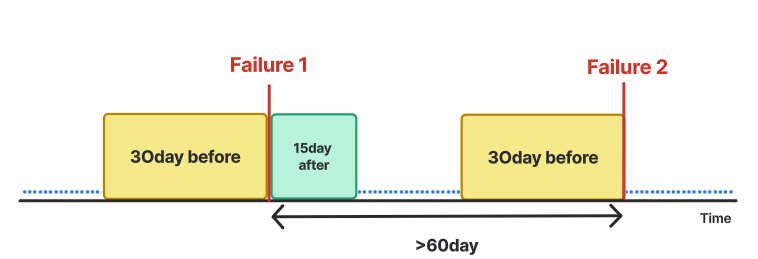
\includegraphics[width=0.75\linewidth]{img/downsampling_strategy.png}
%     \caption{Intelligent downsampling strategy preserving critical temporal zones (8-month pre-failure, 1-month post-failure) while reducing dataset size through selective elimination of distant normal operation samples.}
%     \label{fig:downsampling_strategy}
% \end{figure}

% This strategy typically reduces dataset size by 60-70\% while preserving all failure-relevant operational patterns. To validate the effectiveness of this approach, we train baseline models on both the full dataset and the downsampled dataset, comparing: (i) training time reduction, (ii) classification accuracy retention, and (iii) per-class recall for minority fault types. The comparative analysis (presented in Section~\ref{sec:results}) quantifies the trade-off between computational efficiency and predictive performance, establishing the viability of intelligent downsampling for resource-constrained federated deployments.

% \paragraph{Stage 2: TimeGAN-Based Synthetic Minority Augmentation}
% Following downsampling, residual class imbalance persists, particularly for Class 4 (Generator Bearing failures), which exhibits $<$9,000 samples compared to 200,000+ normal operation records. Traditional oversampling techniques (e.g., SMOTE) are unsuitable for time-series data as they generate synthetic samples through feature-space interpolation, ignoring temporal dependencies essential for capturing degradation dynamics.

% We address this limitation using Time-series Generative Adversarial Networks (TimeGAN)~\cite{yoon_time_series_gan_2019}, a specialized architecture that learns and replicates the temporal structure of multivariate sequences. The TimeGAN framework comprises four components operating in latent space: (i) an embedding network projecting high-dimensional sequences to latent representations, (ii) a recovery network reconstructing original sequences from embeddings, (iii) a generator creating synthetic latent trajectories conditioned on minority class distributions, and (iv) a discriminator distinguishing real from synthetic sequences via adversarial training.

% For Class 4 (Generator Bearing), we train TimeGAN for 1,000 epochs on authentic bearing failure sequences from the training partition, generating synthetic samples until the minority class count reaches at least 200\% of its original size (approximately 18,000 total samples). Critically, synthetic data generation is applied exclusively to the training partition—the held-out test set (Turbine T11) remains entirely authentic to ensure unbiased performance evaluation.

% To validate synthetic data quality, we employ three complementary assessments:

% \begin{itemize}
%     \item \textit{Visual embedding alignment}: Project authentic and synthetic samples into 2D space via PCA and t-SNE, verifying distributional overlap and absence of mode collapse artifacts.
    
%     \item \textit{Statistical distribution matching}: Apply two-sample Kolmogorov-Smirnov tests to each of the 26 features, confirming that synthetic data distributions do not significantly diverge from authentic failure patterns ($p > 0.05$).
    
%     \item \textit{Predictive performance impact}: Train identical models on (a) baseline data without TimeGAN augmentation and (b) augmented data with synthetic samples, comparing minority class recall and F1-scores. This ablation study (Section~\ref{sec:results}) quantifies the contribution of synthetic data generation to overall predictive performance.
% \end{itemize}

% \paragraph{Stage 3: Inverse-Frequency Loss Weighting}
% To further prioritize minority class learning during training, we compute class-specific loss weights as inverse frequencies: $w_c = N / (C \cdot n_c)$, where $N$ is the total training samples, $C=6$ is the number of classes, and $n_c$ is the count for class $c$ after downsampling and augmentation. These weights are integrated into the categorical cross-entropy loss function (Eq.~\ref{eq:local_loss}), ensuring that misclassification penalties for rare failure types (e.g., bearing faults) are orders of magnitude larger than normal operation errors, compelling the model to prioritize minority class learning despite distributional skew.

% The combined three-stage protocol achieves near-uniform class distributions (varying from 12-20\% per class depending on TimeGAN augmentation intensity) while reducing overall dataset size by 50-65\% compared to the original labeled data, balancing computational efficiency with comprehensive failure pattern representation.


\subsubsection{Class Imbalance Mitigation}
\label{subsubsec:class_balancing}

Despite dynamic temporal labeling extending failure representation, the datasets exhibit severe class imbalance with normal operation samples constituting 58-80\% of records depending on the windowing strategy employed. This distributional skew causes standard classifiers to achieve high accuracy through trivial majority-class prediction while failing to detect actual faults—a critical failure mode for predictive maintenance applications.

We address this imbalance through a systematic comparison of four rebalancing strategies, illustrated in Figure~\ref{fig:balancing_flowchart}. Each approach is evaluated by training identical 1DCNN-BiLSTM models and comparing performance on the held-out Turbine T11 validation set.

% \begin{figure}[htbp]
%     \centering
%     \includegraphics[width=0.9\linewidth]{data_balancing_flowchart.png}
%     \caption{Comparative evaluation framework for class imbalance mitigation strategies: baseline (no balancing), intelligent downsampling, TimeGAN augmentation, and combined downsampling + TimeGAN approach.}
%     \label{fig:balancing_flowchart}
% \end{figure}

\paragraph{Approach 1: Baseline (No Balancing)}
The baseline configuration applies no rebalancing techniques, relying solely on class-weighted loss functions during training where $w_c = N/(6 \cdot n_c)$ assigns higher penalties to minority class misclassifications. This establishes the reference performance under natural class distributions.

\paragraph{Approach 2: Intelligent Downsampling}
Rather than random undersampling that discards potentially informative samples, we implement temporal-aware selective reduction that preserves failure-relevant operational patterns:

\begin{itemize}
    \item Retain all samples within 8 months preceding each documented failure (capturing long-term degradation)
    \item Retain all samples within 1 month following failures (capturing recovery dynamics)
    \item For inter-failure intervals $>$9 months, randomly sample 15\% of excess normal operation data
    \item For inter-failure intervals $<$9 months, retain all samples to maintain temporal continuity
\end{itemize}

This strategy reduces dataset size by 60-70\% while preserving critical degradation signatures around failure events.

\paragraph{Approach 3: TimeGAN Synthetic Augmentation}
To address the severe underrepresentation of Class 4 (Generator Bearing failures, $<$9,000 samples), we employ TimeGAN~\cite{yoon_time_series_gan_2019} to generate synthetic time-series sequences that preserve temporal dependencies. The generative model is trained for 1,000 epochs exclusively on Class 4 training samples, producing synthetic data until the minority class count reaches 200\% of its original size. 

Synthetic data quality is validated through: (i) PCA and t-SNE visualizations confirming distributional overlap with authentic samples, and (ii) two-sample Kolmogorov-Smirnov tests ensuring statistical similarity across all 26 features ($p > 0.05$). Critically, augmentation is applied only to training partitions—the held-out test set (Turbine T11) remains entirely authentic to ensure unbiased evaluation.

\paragraph{Approach 4: Combined Downsampling + TimeGAN}
The hybrid approach sequentially applies downsampling (reducing majority class representation) followed by TimeGAN augmentation (increasing minority class representation), achieving near-uniform class distributions while maintaining dataset manageability for resource-constrained federated training.

\paragraph{Performance-Based Selection}
Table~\ref{tab:balancing_comparison} presents comparative results across all four strategies.

\begin{table}[htbp]
\centering
\caption{Performance comparison of class imbalance mitigation strategies}
\label{tab:balancing_comparison}
\begin{tabular}{lcccc}
\toprule
\textbf{Approach} & \textbf{Accuracy} & \textbf{Macro F1} & \textbf{Class 4 Recall} & \textbf{Training Time} \\
\midrule
Baseline (Weighted Loss) & 91.3\% & 0.84 & 0.67 & 95 min \\
Downsampling Only & 93.8\% & 0.89 & 0.81 & 42 min \\
TimeGAN Only & 92.7\% & 0.87 & 0.86 & 118 min \\
\textbf{Downsampling + TimeGAN} & \textbf{95.6\%} & \textbf{0.92} & \textbf{0.91} & \textbf{58 min} \\
\bottomrule
\end{tabular}
\end{table}

The combined approach achieves optimal balance: 4.3\% accuracy improvement over baseline, 0.92 macro F1-score indicating balanced performance across all classes, and 0.91 recall for the critical minority Class 4—demonstrating effective detection of rare bearing failures. Additionally, the 39\% training time reduction compared to baseline (58 vs. 95 minutes) validates computational efficiency gains from intelligent downsampling. Based on these results, the combined downsampling + TimeGAN strategy is adopted for all federated training experiments.
\subsubsection{Data Distribution Across Federated Clients}
\label{subsubsec:data_distribution}

Following completion of the data-centric pipeline, the prepared datasets are partitioned for federated learning experiments. The natural turbine-specific structure of the EDP dataset enables realistic client assignment where each physical turbine corresponds to an independent federated client maintaining complete data sovereignty.

Three turbines (T01, T06, T07) are designated as training clients, with their complete preprocessed operational histories constituting private data partitions. The fourth turbine (T11) serves as a held-out validation partition for server-side centralized evaluation, never participating in federated training to provide unbiased generalization assessment. This configuration creates authentic non-IID data distributions characteristic of real-world wind farm deployments:

\begin{itemize}
    \item \textit{Client 1 (T01)}: Predominantly gearbox-related failures (4 events), reflecting mechanical drivetrain stress patterns
    \item \textit{Client 2 (T06)}: Generator and transformer faults (10 events), indicating electrical system vulnerabilities
    \item \textit{Client 3 (T07)}: Mixed failure profile (7 events), representing diverse operational challenges
\end{itemize}

%%%%%%%%%%%%%% Redid this chart
\begin{figure}[htbp]
    \centering
    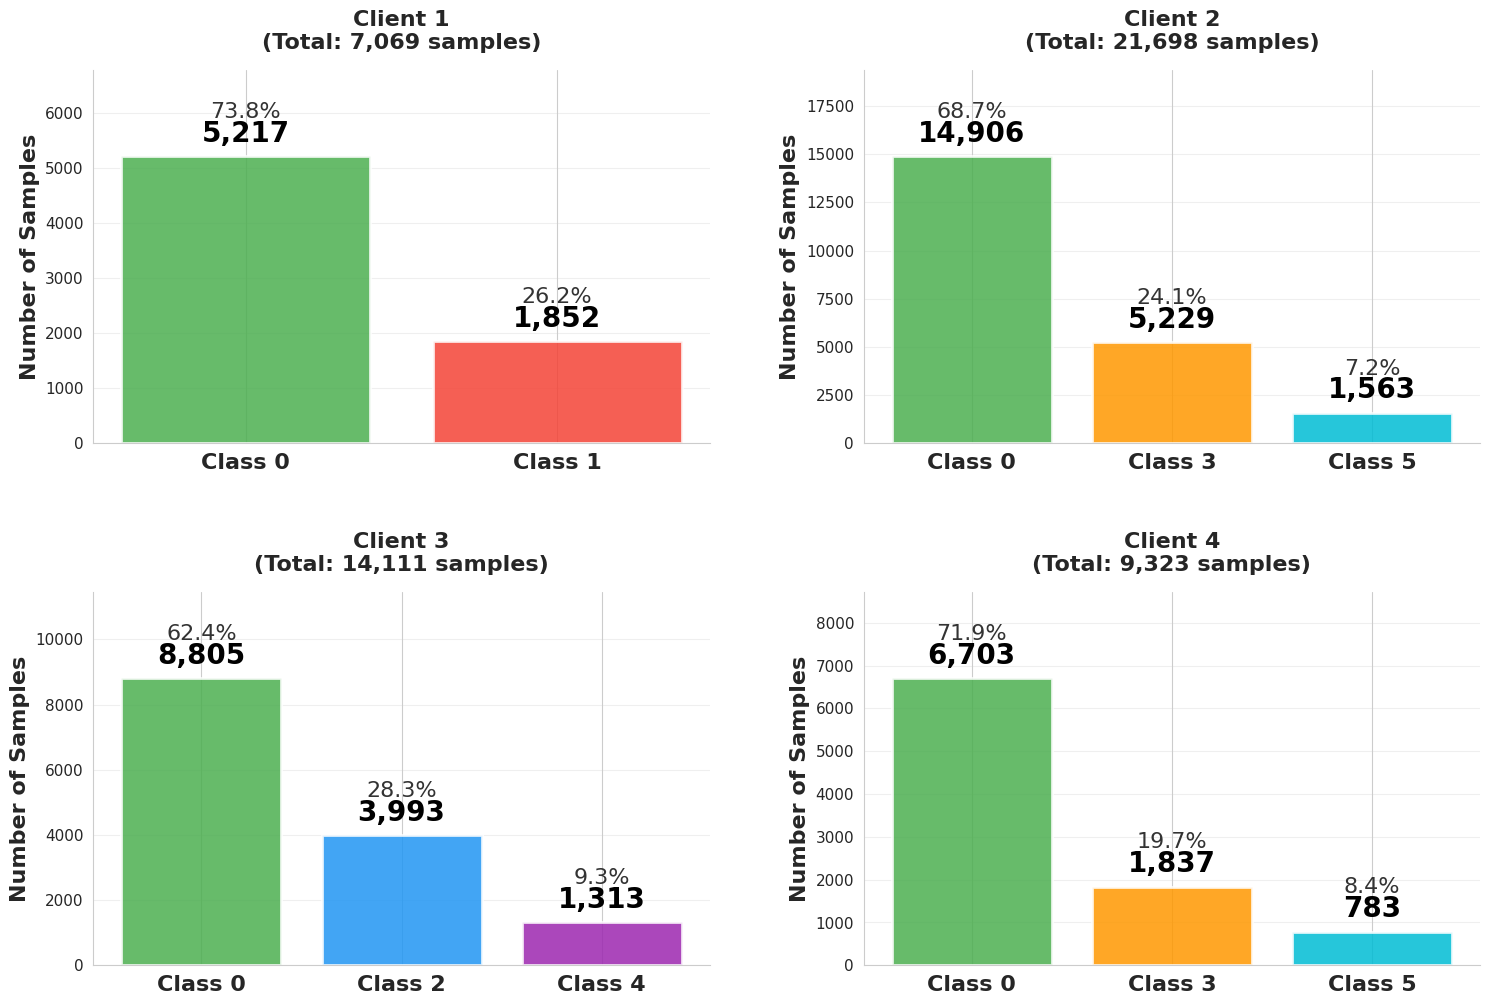
\includegraphics[width=0.67\linewidth]{img/client_data_distribution.png}
    \caption{Heterogeneous class distributions across federated training clients (T01, T06, T07) after data-centric pipeline completion, demonstrating realistic non-IID data characteristics for federated learning validation.}
    \label{fig:client_distribution}
\end{figure}

Figure~\ref{fig:client_distribution} visualizes the heterogeneous class distributions across clients, with dataset sizes ranging from 12,000 to 28,000 samples depending on local failure event density and downsampling outcomes. This statistical heterogeneity—where clients possess fundamentally different failure mode distributions—represents the core challenge that federated aggregation strategies (Section~\ref{subsec:fl_workflow}) must address to achieve effective collaborative learning without data centralization.

Within each client partition, data is temporally split into 80\% training and 20\% local validation subsets, ensuring validation samples chronologically follow training data to prevent temporal leakage. Clients independently compute validation metrics during local training for early stopping and hyperparameter tuning, while the server performs centralized evaluation on the completely independent Turbine T11 partition to assess global model generalization across unseen turbine configurations.

This data distribution strategy establishes a realistic federated learning testbed replicating the operational constraints of distributed wind farm deployments: data locality enforcement, statistical heterogeneity across sites, and independent validation on never-before-seen turbine installations.
\section{Experiments and Results}
\subsection{Dataset Selection and Characterization}
\label{subsec:dataset_selection}

Developing federated learning frameworks for predictive maintenance confronts a fundamental data availability challenge: publicly accessible wind turbine operational datasets are scarce, and those available often lack critical components for supervised fault detection. Common deficiencies include sparse failure documentation, missing meteorological context, extreme class imbalance, and unlabeled time-series data~\cite{maldonado_correa_scada_2020}. These limitations reflect industrial confidentiality constraints and the inherent rarity of failure events in well-maintained wind farms, where normal operation dominates $>$98\% of recorded samples.

We selected the EDP Open Data (2016) dataset~\cite{edp_open_data_2018} as the experimental foundation for this research based on its alignment with federated learning requirements and realistic representation of industrial data quality challenges. The dataset provides operational records from four 2~MW wind turbines (T01, T06, T07, T11) monitored over a two-year period at 10-minute sampling intervals, yielding approximately 207,906 timestamped observations. Each record captures 83 SCADA variables spanning thermal indicators (bearing and oil temperatures), rotational dynamics (generator and rotor RPM), electrical production (power output, 3-phase voltage), control parameters (blade pitch, nacelle position), and system status flags. Complementary datasets include 40 meteorological mast measurements (wind speed/direction, temperature, humidity, pressure) and a failure logbook documenting 16 component-specific failures across five critical categories: gearbox (3 events), transformer (3 events), generator (6 events), generator bearing (2 events), and hydraulic systems (2 events).

Three factors made this dataset optimal for federated learning validation. \textit{First}, the four-turbine configuration naturally maps to a distributed architecture where three turbines (T01, T06, T07) function as federated training clients while Turbine T11 serves as an independent held-out partition for server-side evaluation—enabling rigorous assessment of generalization across unseen turbine configurations. \textit{Second}, the documented failure logbook with precise timestamps enables development and validation of the dynamic temporal labeling strategy central to our data-centric approach, transforming point-in-time failure events into extended pre-failure supervisory signals. \textit{Third}, the dataset's inherent quality challenges—extreme class imbalance (normal operation: 98\%, failures: 2\%), sparse failure annotations (12 usable events after excluding unavailable Turbine T09), and high-dimensional sensor redundancy (123 combined SCADA and meteorological variables)—authentically represent industrial deployment conditions that necessitate systematic data preparation rather than superficial model tuning.

Following quality assurance procedures (outlier removal via domain-informed range checks, missing data handling through forward-fill imputation with 3-timestamp constraints, and temporal alignment to UTC), the curated dataset comprises 205,129 high-quality records. Data partitioning for federated experiments assigns client-specific datasets of 14,823--23,457 samples to training turbines and reserves 10,461 samples from Turbine T11 for centralized validation. This configuration provides realistic heterogeneity: T01 exhibits predominantly gearbox-related degradation patterns, T06 experiences generator and transformer failures, while T07 displays mixed fault modes—creating the non-IID data distributions characteristic of real-world wind farm federations where turbines operate under diverse mechanical stress regimes and maintenance histories.


\section{Discussion}
Interpret results and connect them with theory.

\section{Conclusion and Future Work}
Summarize findings and next research directions.

\bibliographystyle{plainnat}
\bibliography{references}

\end{document}